\chapter{Lecture}\label{part1:lec7}
\markboth{\thechapter. Lecture}{\thechapter. Lecture}

We \pageoriginale wish to say something about the celebrated
Rogers-Ramanujan identities:
\begin{align*}
  1 + \frac{x}{1-x} + \frac{x^4}{(1-x)(1-x^2)} +
  \frac{x^9}{(1-x)(1-x^2)(1-x^3)} \\
  +\cdots \qquad =
  \frac{1}{\substack{\prod\\n>0\\n \equiv \pm 1
      \pmod{5}}(1-x^n)};\tag{1}\label{part1:lec7:eqq1} \\
  1+ \frac{x^2}{1-x}+ \frac{x^{2\cdot 3}}{(1-x)(1-x^2)} +
  \frac{x^{3\cdot 4}}{(1-x)(1-x^2)(1-x^3)}\\
  + \cdots \qquad  = 
 \frac{1}{\substack{\prod\\n>0\\n \equiv \pm 2 \pmod{5}}(1-x^n)}
 \tag{2}\label{part1:lec7:eqq2} 
\end{align*}

The right hand sides of (\ref{part1:lec7:eqq1}) and
(\ref{part1:lec7:eqq2}), written  down explicitly, are respectively
\begin{gather*}
  \frac{1}{(1-x)(1-x^4)(1-x^6)(1-x^9)\ldots}\\
  \frac{1}{(1-x^2)(1-x^3)(1-x^7)(1-x^8)\ldots}
\end{gather*}

One immediately observes that $\pm 1$ are quadratic residues modulo 5,
and $\pm 2$ quadratic non-residues modulo 5. These identities were
first communicated by Ramanujan in a letter written to Hardy from
India in February 1913 before he embarked for England. No proofs were
given at that time. It was a remarkable fact, nevertheless, to have
even written\pageoriginale down such identities. It is true that
Euler himself did some experimental work with the pentagonal numbers
formula. But one does not see the slightest reason why anybody should
have tried $\pm 1$, $\pm 2$ modulo 5. Then in 1917 something
happened. In an old volume of the Proceedings of the London
Mathematical Society Ramanujan found that Rogers (1894) had these
identities along with extensions of hypergeometric functions and a
wealth of other formulae. In 1916 the identities were published in
Macmahon's Combinatory Analysis without proof, but with a
number-theoretic explanation. This was some progress. In 1917 I.Schur
gave proofs, one of them combinatorial, on the lines of F.Franklin's
proof of Euler's theorem. Schur also emphasized the mathematical
meaning of the identities. 

Let us look at the meaning of these identities. Let us write the right
side of (\ref{part1:lec7:eqq1}) as a power-series, say, 
$$
  \frac{1}{(1-x)(1-x^4)(1-x^6)(1-x^9)\ldots}= \sum^\infty_{n=0} q'(n) x^n,
$$
$q'(n)$ is the number of terms collected from summands 1, 4, 6,
  $\ldots$ with repetitions, or, what is the same thing, the number of
  times in which $n$ can be expressed as the sum of parts $\equiv \pm
  1 \pmod{5}$, with repetitions. Likewise, if we write
$$
  \frac{1}{\prod\limits_{n \equiv \pm 2(5)}(1-x^n)} = \sum^\infty_{n=0}
  q''(n) x^n,
$$
then $q''(n)$ is the number of representations of $n$ as the sum of
parts $\equiv \pm 2 \pmod{5}$, with repetitions.

The expressions on the other side appear directly.

Take\pageoriginale 
$$
\frac{x^{k^2}}{(1-x)(1-x^2)\cdots (1-x^4)}
$$

If we write
$$
\frac{1}{(1-x)(1-x^2)\cdots (1-x^k)}= a_0 + a_1 x + a_2x^2+ \cdots
$$
then the coefficient $a_n$ gives us the number of partitions of $n$
into parts not exceeding $k$. Let us represent the partitions by dots
in a diagram, each vertical column denoting a summand. Then there are
at most $k$ rows in the diagram. Since $k^2$ is the sum of the $k$
first odd numbers,
$$
k^2 =1+ 3+5+ \cdots + (2k-1),
$$
each partition of $n$ into summands not exceeding $k$ can be enlarged
into a partition of $n+k^2$ into summands which differ by at least
two, for we can adjoin $k^2$ dots on the left side, putting one in the
lowest row, three in the next, five in the one above and so on finally
$2k-1$ in the top most row. Conversely any partition of $n$ into 

\begin{figure}[H]
  \centering{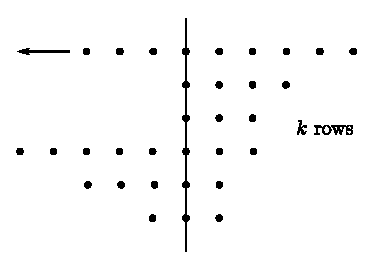
\includegraphics{vol2-figures/fig2.12.eps}}
\end{figure}
\noindent parts with minimal difference 2 can be mutilated into a partition
of\pageoriginale $n-k^2$ into summands not exceeding $k$. Hence there
is a one one correspondence between these two types. So the
coefficients in the expansion of\break $\dfrac{x^{k^2}}{(1-x)(1-x^2)\cdots
  (1-x^k)}$ represent the number of times that a number $N$ can be
decomposed into $k$ parts (the partitions are now read horizontally in
the diagram) differing by two at least. When this is done for each $k$
and the results added up, we get the following arithmetical
interpretation of (\ref{part1:lec7:eqq1}): The number of partitions of $n$ with minimal
difference two is equal to the number of partitions into summands
congruent to $\pm 1 \pmod{5}$ allowing repetitions. 

A similar explanation is possible in the case of (\ref{part1:lec7:eqq2}). On the left side
we can account for the exponents 2.3, 3.4, $\ldots$, $k(k+1)$,
$\ldots$ in the numerator by means of triangular numbers. In the
earlier diagram we adjoin on the left 2, 4, 6, $\ldots$, $2k$ dots
beginning with the lowest row. The number thus added is $2+4+\cdots
\cdots \cdots + 2k = k(k+1)$; this disposes of $x^{k(k+1)}$in the
  numerator. So read horizontally, the diagram gives us a
  decomposition into parts which differ by 2 at least, but the summand
  1 is no longer tolerated. $\dfrac{x^{k(k+1)}}{(1-x)\cdots (1-x^k)}$
  gives us therefore the enumeration of $x^N$ by parts differing by 2
  at least, the part 1 being forbidden. We have in this way the
  following arithmetical interpretation of (\ref{part1:lec7:eqq2}): The number of
  partitions of $n$ into parts not less than 2 and with minimal
  difference 2, is equal to the number of partitions of $n$ into parts
  congruent $\pm 2 \pmod{5}$, repetitions allowed.

By\pageoriginale a similar procedure we can construct partitions
where 1 and 2 are forbidden, partitions differing by at least three,
etc. In the case where the difference is 3, we use $1, 4, 7, \ldots$,
so that the number of dots adjoined on the left is $1+4+7+\cdots$ to
$k$ terms $= k(3k-1)/2$, so a pentagonal number, and this is no
surprise. In fact $\sum \dfrac{x^{k(3k-1)/2}}{(1-x)(1-x^2)\cdots
  (1-x^k)}$ would give us the number of partitions into parts
differing by at least 3. And for 4 the story is similar.

The unexpected element in all these cases is the association of
partitions of a definite type with divisibility properties. The
left-side in the identities is trivial. The  deeper part is the right
side. It can be shown that there can be no corresponding identities
for moduli higher than 5. All these appear as wide generalisations of
the old Euler theorem in which the minimal difference between the
summands is, of course, 1. Euler's theorem is therefore the nucleus of
all such results.

We give here a proof of the Roger-Ramanujan identities which is in
line with the treatment we have been following, the method of formal
power series. It is a transcription of Roger's proof in Hardy's
`Ramanujan', pp.95-98. We use the so-called Gaussian polynomials.

Let us introduce the Gaussian polynomials in a much neater notation
than usual. Consider for first the binomial coefficients:
$$
\binom{n}{m} = \frac{n(n-1)(n-2) \cdots (n-k+1)}{1 \cdot 2 \cdot
  3\cdot \cdots k}
$$

(Observe\pageoriginale that both in the numerator and in the
denominator there are $k$ factors, which are consecutive integers, and
that the factors of equal rank in both numerator and denominator
always add up to $n+1$). The $\binom{n}{k}$ are all integers, as is
obvious from the recursion formula
$$
\binom{n+1}{k} = \binom{n}{k} + \binom{n}{k-1}
$$
$\binom{n}{n}=1$, of course, and by definition, $\binom{n}{0}=1$ We
also define $\binom{n}{k} =0$ for $k > n$ or for $k<0$. Observe also
the symmetry: $\binom{n}{k} = \binom{n}{n-k}$

The Gaussian polynomials are something of a similar nature. We define
the Gaussian polynomial
$$
\displaylines{\hfill 
\begin{bmatrix}n\\k\end{bmatrix}= 
\begin{bmatrix}n\\k\end{bmatrix}_x\hfill \cr
\text{by} \hfill  \begin{bmatrix}n\\k\end{bmatrix} =
  \frac{(1-x^n)(1-x^{n-1})\cdot (1-x^{n-k+1})}{(1-x)(1-x^2)\cdots
    (1-x^k)} \hfill }
$$

The sum of the indices of $x$ in corresponding factors in the
numerator $r$ and denominator is $n+1$, as in $\binom{n}{k}$. That
the $\begin{bmatrix}n\\k\end{bmatrix}$ are polynomials in $x$ is
  obvious from the recursion formula
$$
\begin{bmatrix}n+1\\k\end{bmatrix}
  = \begin{bmatrix}n\\k\end{bmatrix}+ \begin{bmatrix}n+1\\k-1\end{bmatrix}
      x^k  
$$  
where $\begin{bmatrix}n\\n\end{bmatrix}=1$ and
  $\begin{bmatrix}n\\0\end{bmatrix}=1$ by definition. The recursion
    formula is just the same as that for $\binom{n}{k}$ except for the
    factor in the second term on the right. Also define
    $\begin{bmatrix}0\\0\end{bmatrix}=1$; also\pageoriginale let
      $\begin{bmatrix}n\\0\end{bmatrix}=1$ for $k>n$ or $k<0$.
\begin{align*}
  \begin{bmatrix}1\\0\end{bmatrix} &
    = \begin{bmatrix}0\\0\end{bmatrix}+ \begin{bmatrix}0\\-1\end{bmatrix}
        x^\circ =1,\\
  \begin{bmatrix}1\\1\end{bmatrix} &
    = \begin{bmatrix}1\\0\end{bmatrix};\\
  \begin{bmatrix}2\\1\end{bmatrix} & = \frac{1-x^2}{1-x} = 1+x;   
\end{align*}
and so on. We also have the symmetry:
$$
\begin{bmatrix}n\\k\end{bmatrix}= \begin{bmatrix}n\\n-k\end{bmatrix}
$$

The binomial coefficients appear in the expansion
$$
(1+ y)^2= \sum\limits^n_{k=0} \binom{n}{k} y^k.
$$

Likewise, the Gaussian polynomial $\begin{bmatrix}n\\k\end{bmatrix}$
  appear in expansion:
$$
\displaylines{\hfill (1+y)(1+xy) (1+x^2y) \cdots (1+x^{n-1}y) = 1+y
  G_1 (x) + y^2 G_2 (x) + \cdots + y^n G_n (x)\hfill \cr
  \text{where} \hfill G_k(x) =
  x^{k(k-1)/2} \begin{bmatrix}n\\k\end{bmatrix} \hfill }
$$

Notice that for $x=1$, $\begin{bmatrix}n\\k\end{bmatrix}=
  \binom{n}{k}$. Changing $y$ to $yx$ we get the recursion formula
  stated earlier.

We now go back to an identity we has proved sometime back:
\begin{equation*}
\prod^\infty_{n=1} (1+ \mathfrak{z}x^{2n-1}) = 1
  + \mathfrak{z} C_1 (x) + \mathfrak{z}^2 C_2 (x) +
  \cdots\tag{1}\label{part1:lec7:eq1} 
\end{equation*}
where
\begin{equation*}
  C_k (x) = \frac{x^{k^2}}{(1-x^2)\cdots (1-x^{2k})} 
\end{equation*}

Now\pageoriginale write
\begin{multline*}
  x^2 = X, 1-X= X_1-X^2 = X_2, \ldots , 1-X^k= X_k;\\
  (1-X)(1-X^2)\cdots (1-X^k)= X, X_2 \ldots X_k = X_k!
\end{multline*}

With this notation,
$$
C_k (x) = \frac{x^{k^2}}{X_k!}
$$

From Jacobi's triple product formula, we have 
\begin{equation*}
  \prod^\infty_{n=1} (1+ \mathfrak{z} x^{2n-1})(1+ \mathfrak{z}^{-1}
  x^{2n-1}) = \frac{\sum\limits^\infty_{\ell =-\infty} \mathfrak{z}^l
    x^{l^2}}{\prod\limits^\infty_{n=1} (1-x^{2n})} \tag{2}\label{part1:lec7:eq2}
\end{equation*}

By (\ref{part1:lec7:eq1}), the left side of (\ref{part1:lec7:eq2}) becomes
$$
\sum^\infty_{r=0} \mathfrak{z}^r C_r (x) \sum^\infty_{s=0}
\mathfrak{z}^{-s} C_s (x) = \sum^\infty_{n=0} \frac{B_n (\mathfrak{z},
  x)}{X_n!}, 
$$
where $X_\circ !$ is put equal to 1. $B_n (\mathfrak{z}, x)$ is the
term corresponding to $r+s=n$ when the left side is multiplied out in
Cauchy fashion. Thus
\begin{align*}
  B_n (\mathfrak{z}, x) & = X_n ! \sum_{r+s=n} \mathfrak{z}^{r-s} C_r
  (x) C_s (x)\\
  & = X_n ! \sum^n_{r=0} \mathfrak{z}^{n-2r} \frac{x^{r^2+s^2}}{X_r!
    X_{n-r}!}~(r+s=n)\\
  & = \sum^n_{r=0} \begin{bmatrix} n\\r \end{bmatrix}_X x^{(n-r)^2+
    r^2} \mathfrak{z}^{n-2r}
\end{align*}

Notice\pageoriginale that the powers of $z$ occur with the same
parity as $n$. Now (\ref{part1:lec7:eq2}) can be re-written as 
$$
\sum^\infty_{n=0} \frac{B_n(\mathfrak{z}, x)}{X_n!} =
\frac{\sum\limits^\infty_{l=-\infty} \mathfrak{z}^l
  x^{l^2}}{\prod\limits^\infty_{n=1} (1- x^{2n})}
$$ 

Both sides are formal power series in $x$ of the appropriate sort. The
$B_n(\mathfrak{z}, x)$ are linear combinations of power series in $x$
with powers of $z$ for coefficients. We can now compare powers of
$z$. We first take only even exponents $\mathfrak{z}^{2m}$; we then
have infinitely many equations of formal power series. We multiply the
equation arising from $\mathfrak{z}^{2m}$ by $(-)^m x^{m(m-1)}$ and
add all these equations together; (and that is the trick, due to
Rogers) we can do this because of linearity. Then
\begin{align*}
\sum^\infty_{l=0} \frac{\beta_{2l} (x)}{X_{2l}!} & =
  \frac{\sum\limits^\infty_{m=0} (-)^m
    x^{m(m-1)}x^{(2m)^2}}{\prod\limits^\infty_{n=1}
    (1-x^{2n})},\tag{3}\label{part1:lec7:eq3} \\
  \text{where} \hspace{1cm} \beta_{2l} (x) & =
  \sum^{2l}_{r=0} \begin{bmatrix}2l\\r\end{bmatrix}_X x^{(2l -r)^2 +
      r^2} (-)^{l-r}x^{(l-r)(l-r-1)}\hspace{1cm}
\end{align*}

Writing $l-r=s$, 
\begin{align*}
  \beta_{2l} (x) & = \sum^l_{s=-l} \begin{bmatrix}
    2l\\l-s \end{bmatrix} x^{2l^2 + 2s^2} (-)^s x^{s(s-1)}\\
  & = x^{2l^2} \sum^l_{s=-l} \begin{bmatrix} 2l\\ l+s \end{bmatrix}
  (-)^s x^{3 s^2} -s 
\end{align*}
(because of the symmetry between $l-s$ and $l+s$). Separating out the
term corresponding  to $s=0$ and folding together the
terms\pageoriginale corresponding to $s$ and $-s$,
\begin{align*}
  \beta_{2l}(x) & = x^{2l^2} \left\{ \begin{bmatrix}
    2l\\l\end{bmatrix} + \sum^l_{s=1} (-)^s \begin{bmatrix}
      2l\\l+s \end{bmatrix} x^{s(3s-1)} (1+x^{2s})\right\}\\
    & = x^{2l^2} \left\{ \sum^l_{s=1}
    (-)^s \begin{bmatrix}2l\\l+s\end{bmatrix} x^{s(3s-1)}+
      \sum^l_{s=0} (-)^s \begin{bmatrix} 2l\\l+s \end{bmatrix}
      x^{s(3s+1)}\right\}\\
      & = x^{2l^2} \left\{ \sum^l_{s=0} (-)^{s+1} \begin{bmatrix}
        2l\\l+s+1 \end{bmatrix} x^{(s+1) (3s+2)} + \sum^l_{s=0}
      (-)^s \begin{bmatrix} 2l\\l+s\end{bmatrix} x^{s(3s+1)} \right\}
        \tag{4}\label{part1:lec7:eq4} 
\end{align*}

Then
\begin{align*}
  \beta_{2l} (x) & = x^{2l^2} \sum^l_{s=0} (-)^s\begin{bmatrix}
  2l\\l+s\end{bmatrix} x^{s(3s+1)} \left( 1-
  \frac{1-X^{l-s}}{1-X^{l+s+1}} x^{4s+2} \right)\\
  & = x^{2l^2} \sum^l_{s=0} (-)^s \begin{bmatrix} 2l\\l+s\end{bmatrix}
    x^{s(3s+1)} \frac{1-X^{2s+1}}{1-X^{l+s+1}}\\
    & = \frac{x^{2l^2}}{1-X^{2l+1}} \sum^l_{s=0} (-)^s \begin{bmatrix}
      2l+1\\l+s+1\end{bmatrix} x^{s(3s+1)} (1-x^{4s+2})
      \tag{5}\label{part1:lec7:eq5} 
\end{align*}

Let us now compute $\beta_{2l+1}(x)$. For this we compare the
coefficients of $\mathfrak{z}^{2m+1}$, multiply the resulting
equations by $(-)^m x^{m(m-1)}$ and add up. Then
\begin{equation*}
  \sum^\infty_{l=0} \frac{\beta_{2l+1}(x)}{X_{2l+1}!} =
  \frac{\sum\limits^\infty_{m=0} (-)^m x^{m(m-1)}
    x^{(2m+1)^2}}{\prod\limits^\infty_{n=1} (1- x^{2n})},
  \tag{6}\label{part1:lec7:eq6} 
\end{equation*}
where\pageoriginale
\begin{equation*}
  \beta_{2l+1}(x) = \sum^{2l+1}_{r=0} \begin{bmatrix}
    2l+1\\r\end{bmatrix}x^{(2l+1-r)^2} + r^2 (-)^{l-r} x^{(l-r) (l-r-1)}
\end{equation*}

Writing $l-r=s$, this gives
\begin{align*}
  \beta_{2l+1}(x) & = \sum^{l}_{s=-l-1} \begin{bmatrix}
    2l+1\\l-s\end{bmatrix}x^{(l+1-s)^2 + (l-s)^2} (-)^{s} x^{s(s-1)}\\
    & = \sum^l_{s=-l-1} \begin{bmatrix} 2l+1\\l-s \end{bmatrix} (-)^s
    x^{3s^2 +s + l^2+(l+1)^2}\\
    & = x^{2l^2 +2l +1} \left\{\sum^l_{s=0} (-)^s \begin{bmatrix}
      2l+1\\l+s+1\end{bmatrix} x^{s(3s+1)}\right.\\
      & \hspace{2cm}\left.+ \sum^l_{s=0}
      (-)^{s+1} \begin{bmatrix} 2l+1\\l+s+1\end{bmatrix}
        x^{(-s-1)(-3s-2)} \right\}\\
    & = x^{2l^2 + 2l +1} \sum^l_{s=0} (-)^s 
        \begin{bmatrix}2l+1\\l+s+1\end{bmatrix} x^{s(3s+1)}
          (1-x^{4s+2}) \tag{7}\label{part1:lec7:eq7}   
\end{align*}

This expression for $\beta_{2l+1}(x)$ is very neat; it is almost the
same as $\beta_{2l}(x)$ but for trivial factors. Let us go back to
$\beta_{2l+1} (x)$ in its best shape.
\begin{align*}
  \beta_{2l+1} (x) & = x^{2l^2+ 2l+1}
  \left\{ \begin{bmatrix}2l+1\\l\end{bmatrix}\right.\\ 
    & \left.\qquad + \sum^l_{s=1}
    \left( \begin{bmatrix}2l+1\\l+s+1\end{bmatrix} (-)^s x^{s(3s+1)}
      + \begin{bmatrix}2l+1\\l+s\end{bmatrix} (-)^s
        x^{s(3s-1)}\right)\right\}\\
    & =x^{2l^2+2l +1}\left\{ \begin{bmatrix}2l+1\\l\end{bmatrix} +
          \sum^l_{s=1} \begin{bmatrix}2l+1\\l+s\end{bmatrix} (-)^s
            x^{s(3s-1)} \left(1+ \frac{1
              -X^{l-s+1}}{1-X^{l+s+1}}x^{2s}\right)\right\} 
\end{align*}
Since\pageoriginale
\begin{align*}
  1+ \frac{1-X^{l-s+1}}{1-X^{l+s+1}} x^{2s} & = \frac{1-X^{l+s+1}+ X^s
    - X^{l+1}}{1-X^{l+s+1}} =
  \frac{(1-X^{l+1})(1+X^s)}{1-X^{l+s+1}},\\
  \beta_{2l+1} (x) & = x^{2l^2+2l+1} \frac{1-X^{l+1}}{1-X^{2l+2}}\\
  &\qquad  \left\{ \begin{bmatrix}2l+2\\l+1\end{bmatrix} + \sum^{l+1}_{s=1} 
    \begin{bmatrix}2l+2\\l+s+1\end{bmatrix} (-)^s x^{s(3s-1)} (1+x^{2s})\right\}
\end{align*}

This fits with $\beta_{2l+2}$. Now we can read off the recursion
formulae. The consequences are too very nice facts. The whole thing
hinges upon the courage to tackle these sums. We did not do these
things ad hoc.

Let us compare $\beta_{2l+1}$ with $\beta_{2l}$
\begin{align*}
  \beta_{2l+1} & = x^{2l+1} (1-X^{2l+1}) \beta_{2l};\\
  \beta_{2l+1} & = x^{-2l-1} \frac{1-X^{l+1}}{1-X^{2l+2}}
  \beta_{2l+2};\\
  \text{so} \hspace{3cm} \beta_{2l+2} & = x^{2l+1}
  \frac{1-X^{2l+2}}{1-X^{l+1}} \beta_{2l+1}, \hspace{3cm}
\end{align*}
and $\beta_\circ =1$. These things collapse beautifully into something
which we could not foresee before. Of course the older proof was
shorter. This proof fits very well into our scheme. 
